
\chapter{Full Connected Networks}
\label{cha:full-conn-netw}

A fully connected neural network consists of a series of fully connected layers that connect every neuron in one layer to every neuron in the other layer.
Full connected neural network layers use matrix multiplication by a matrix of parameters with a separate parameter describing the interaction between each input unit and each output unit.
This means that every output unit interacts with every input unit.


Figure \ref{fig:fc} show the full connects neural network.
\begin{figure}[!htbp]
  \centering
  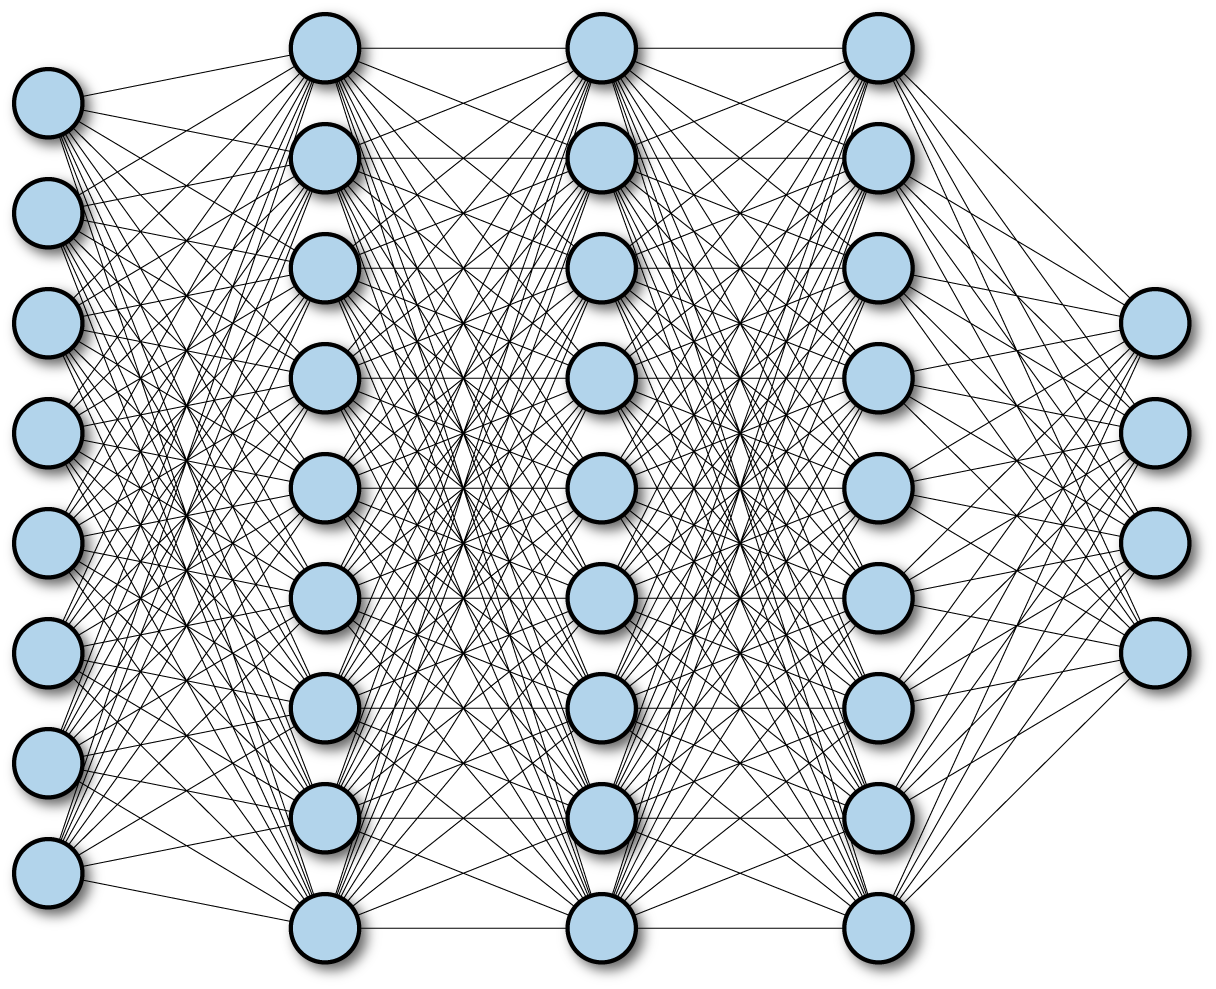
\includegraphics[width=0.8\textwidth]{fc}
  \caption{Full connected neural network}
  \label{fig:fc}
\end{figure}



%%% Local Variables:
%%% mode: latex
%%% TeX-master: "deep-learning"
%%% End:
